\documentclass[]{report}
\usepackage[english]{babel}
\usepackage[backend=bibtex]{biblatex}
\usepackage{graphicx}
\usepackage{float}
\usepackage{hyperref} %[hidelinks]
\usepackage{xcolor}
\usepackage{wrapfig}
\hypersetup{
	colorlinks,
	linkcolor={red!50!black},
	citecolor={blue!50!black},
	urlcolor={blue!80!black}
}

\graphicspath{ {../Img/} }
\addbibresource{../BLDC_ESC_Control_Bib.bib}

% Title Page
\title{	\huge BLDC ESC control \\
		\large Project Proposal \\ 5LIU0}
\author{Enzo Evers}

\pagestyle{plain}

\begin{document}
\maketitle
\tableofcontents

\newpage

\begin{tabular}{|l|l|}
	\hline
	BLDC & Brushless Direct Current \\
	\hline
	BEMF & Back Electromotive Force \\
	\hline
	FOC & Field Oriented Control \\
	\hline
	ESC & Electronic Speed Controller \\
	\hline
	FC & Flight Controller \\
	\hline
	FPV & First Person View \\
	\hline
	RC & Radio Controlled \\
	\hline
	RPM & Rotations Per Minute \\
	\hline
	mRPM & mechanical Rotations Per Minute \\
	\hline
	eRPM & electrical Rotations Per Minute \\
	\hline
\end{tabular}

\newpage

\chapter{Background}
Almost all vehicles in the Radio Control (RC) hobby use a motor of which the speed in controlled using a transmitter. While some cheap (or old) RC vehicles still use brushed DC motors, most of the motors used today are Brushless Direct Current (BLDC) motors. BLDC motors for RC cars are generally bigger then BLDC motors for airplanes or drones but the principle is the same. All BLDC motors require an Electronic Speed Controller (ESC) to be able to be controlled with a microcontroller.

In the (self-build) First Person View (FPV) drone branch of the RC hobby almost all ESCs use the now closed source BLHeli\_32 \cite{BLHeli_Git} firmware. Some current ESCs also use either BLHeli\_S or BLHeli. While these are technically open source, only the assembly sources are available \cite{BLHeli_Git}. A small part of the ESCs use the closed source KISS \cite{KISS_website} firmware. The rest of the current firmwares are either created by the company who also makes the complete drone, are outdated  or are a hobby project.

Firmware for the FPV Flight Controllers (FC) however are almost all open source.

Lately the AM32 \cite{AM32_Git}\cite{AM32_RCGroups} open source ESC firmware project gained some traction. This is a good thing. It is still in development so there are no official products of it yet which can be bought in stores. But once the open source ESC firmware becomes bigger, the price of ESC might go down and innovation in the firmware might accelerate.

That is why, by learning about the guts of the ESC firmware, I want to contribute to the AM32 firmware.

\newpage


\chapter{Goal}

The goal of this project is to create a control system for sensorless BLDC motors used in RC vehicles. Specifically sensorless BLDC motors in First Person View (FPV) drones. To do this, the Back Electromotive Force (BEMF) of the motor is measured and, based on this reading, the motor phases are energized in the correct order. The challenges involved will this are discussed in \autoref{chap:Challenges}. Once the BEMF of the motor can be measured successfully, a control loop will be created to control the speed to the motor. 

While the BEMF method works, a more efficient method would be Field Oriented Control (FOC). This method maximizes the torque and makes the motor spin smoother, resulting in less noise and a higher efficiency \textbf{CITE SOURCE}. This method, however, will not be implemented in the timeframe for this project. FOC is a bit more involved compared to the BEMF method. BEMF sensing is actually one of the components in FOC. By first getting a good understanding of the BLDC control using only the BEMF method, the FOC system implementation becomes easier after that.

Most general ESCs used in the RC hobby don't use FOC anyway. For 

\section{Basic operation of a BLDC motor}
% https://www.instructables.com/Make-Your-Own-Miniature-Electric-Hub-Motor/
\subsection{Six-step commutation}
BLDC motors usually have three phases (most of the time in a star connection) and are, as the name implies, powered by a DC source. Controlling the three phases is done with a six-step commutation system. \autoref{fig:BLDC_SixStep_Table} shows these six steps. The basic idea is that by connecting the DC voltage source in alternating patterns to the phases, the rotating part in the motor (the rotor) which contains the permanent magnets, gets pulled/pushed. Each phase in the stationary part of the motor (the stator) is actually an electromagnets.

\begin{figure}[h]
	\centering
	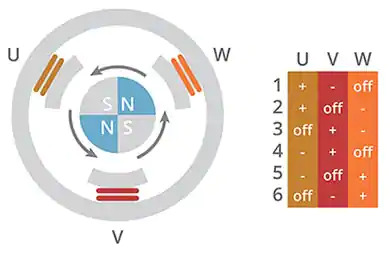
\includegraphics[width=0.5\textwidth]{BLDC_SixStep_Table.jpeg}
	\caption{Table for the six-step commutation \cite{Digikey_BLDC_SixStep}}
	\label{fig:BLDC_SixStep_Table}
\end{figure}

\autoref{fig:BLDC_SixStep_Circuit} shows how this alternating pattern can be implement in hardware. To keep the motor rotating, a feedback loop is needed which measures where the rotor is with respect to the stator and commutates the phases at the correct moment.

\begin{figure}[h]
	\centering
	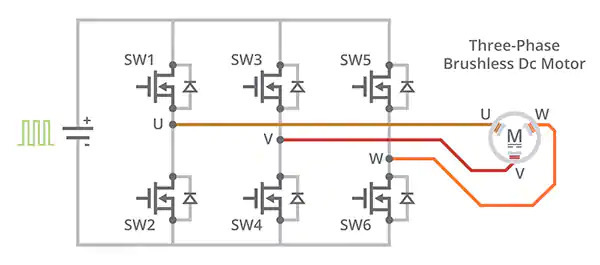
\includegraphics[width=\textwidth]{BLDC_SixStep_Circuit.jpeg}
	\caption{Basic circuit for the six-step commutation \cite{Digikey_BLDC_SixStep}}
	\label{fig:BLDC_SixStep_Circuit}
\end{figure}

\subsection{Inrunner vs outrunner}

Even though the rotor is drawn inside the stator in \autoref{fig:BLDC_SixStep_Table}, it is also possible to have the reverse. When the rotor is inside the stator it is called an inrunner. When the stator is inside the rotor it is called an outrunner (see \autoref{fig:BLDC_Inrunner_VS_Outrunner_Diagram}). RC cars usually use inrunner BLDC motors while drones usually use outrunner BLDC motors. Generally the main difference is that an inrunner has higher RPM but lower torque compared to an outrunner \cite{BLDC_Inrunner_VS_Outrunner}.

\begin{figure}[H]
	\centering
	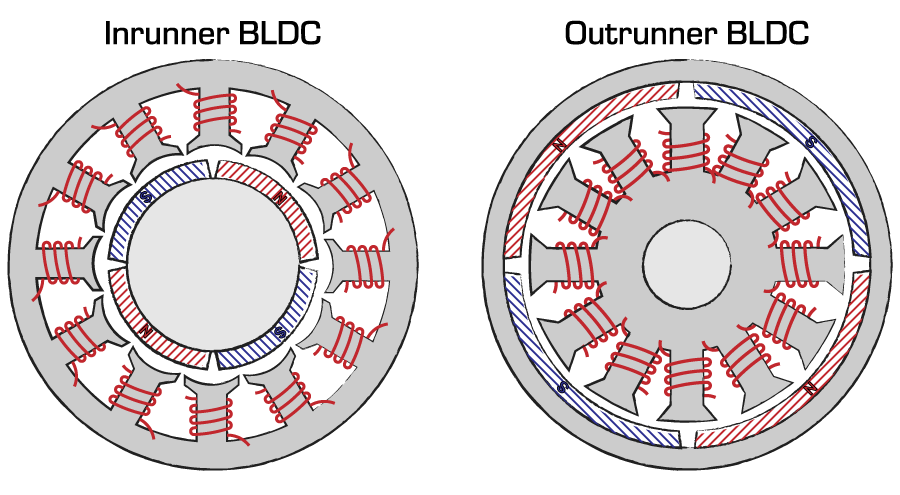
\includegraphics[width=0.75\textwidth]{InOutRunner-2.png}
	\caption{Basic circuit for the six-step commutation \cite{BLDC_Inrunner_VS_Outrunner_Diagram}}
	\label{fig:BLDC_Inrunner_VS_Outrunner_Diagram}
\end{figure}

\subsection{Electrical vs mechanical rotation}

Once all six steps from \autoref{fig:BLDC_SixStep_Table} are executed, one electrical rotation is finished. An electrical rotation is not the same as a mechanical rotation. Depending on the number of permanent magnets there are on the rotor, and how many separate winding there are in the stator for a single phase, (see \autoref{fig:BLDC_Inrunner_VS_Outrunner_Diagram}) one mechanical rotation can consist of one or more electrical rotations.

\section{Changing velocity on RC BLDC motors}
Currently almost all Flight Controllers (FC) and ESCs (Electronic Speed Controller) used in the self-build FPV drones make use of the DShot protocol. This is a serial protocol between the FC and the ESC which sends an 11-bit (2048 steps) throttle value \cite{DShot_Overview}. This throttle value corresponds to the PWM value with which the MOSFETs of the active phases are switched on and off. To make the communication more efficient DShot makes use of the DMA channels of the FC and ESC.

Since the system is powered by a DC source, PWM is a simple method to create a lower average voltage. The reason that DShot is used in most cases is because it is digital. Previously the FC would send an (analogue) PWM/PPM signal to the FC which was susceptible to noise. There is a choice to only apply the PWM signal to the MOSFET connected to the positive terminal of the DC source, or to apply it to both MOSFETs connected to the positive and negative terminals of the DC source. Which method works best needs to be determined.

\section{Inputs and outputs of the system}
\subsection{Flight controller IO (from the ESC's perspective)}
\begin{itemize}
	\item I: Throttle value (11-bit)
	\item O: eRPM (electrical Rotations Per Minute)
\end{itemize}


By default an ESC used in an FPV drone and being controlled with DShot only receives a throttle value from the FC. From version 32.7.0 of BLHeli\_32 and version 4.1 of Betaflight on, RPM (Rotations Per Minute) filtering is implemented. RPM filtering basically tries to eliminate the motor noise in the gyro data. To use RPM filtering bidirectional DShot needs to be enabled. When this is enabled the ESC will report the eRPM in an acknowledgment message on the throttle command from the FC \cite{Betaflight_RPM_Filtering}. Based on the number of permanent magnets in the rotor the mechanical RPM can be calculated.

\subsection{Internal ESC control IO}
\begin{itemize}
	\item O: Six PWM signals to control the MOSFET half-bridges.
	\item I: BEMF
\end{itemize}


\chapter{Challenges} \label{chap:Challenges}
% http://ww1.microchip.com/downloads/en/appnotes/00857a.pdf
% https://www.infineon.com/dgdl/Infineon-TLE987x-Sensorless-Field-Oriented-Control-ApplicationNotes-v01_00-EN.pdf?fileId=5546d46270c4f93e0170f23529817afa
% https://www.youtube.com/watch?v=amt891JwuZ4
% https://www.researchgate.net/publication/321401285_Implementation_of_the_back_EMF_zero_crossing_detection_for_BLDC_motor
% http://educypedia.karadimov.info/library/T.pdf Page 36: 3 sampling points
% https://forum.arduino.cc/index.php?topic=164421.0
% https://www.researchgate.net/publication/319175992_Analysis_of_Position_and_Speed_Control_of_Sensorless_BLDC_Motor_Using_Zero_Crossing_Back-EMF_Technique
% https://www.youtube.com/watch?v=szgVUfyX8JM&t=173s Integraring the BEMF voltage gives flux. InstaSPIN
% https://www.ti.com/lit/ug/spruhj1h/spruhj1h.pdf
% https://www.ti.com/tool/INSTASPIN-BLDC#descriptionArea
% https://www.researchgate.net/publication/319175992_Analysis_of_Position_and_Speed_Control_of_Sensorless_BLDC_Motor_Using_Zero_Crossing_Back-EMF_Technique
% https://toshiba.semicon-storage.com/info/docget.jsp?did=61176
% http://hyperphysics.phy-astr.gsu.edu/hbase/electric/farlaw.html#c1
% https://www.youtube.com/watch?v=7_UDy5PJA8w
% https://www.youtube.com/watch?v=fpTvZlnrsP0
% https://www.researchgate.net/publication/320288579_Modelling_of_a_Sensorless_Rotor_Flux_Oriented_BLDC_machine
% https://www.researchgate.net/publication/228677501_A_New_Approach_to_Sensorless_Control_Method_for_Brushless_DC_Motors
% https://www.st.com/resource/en/application_note/cd00041736-pwm-management-for-3phase-bldc-motor-drives-using-the-st7mc-stmicroelectronics.pdf
% https://www.st.com/resource/en/application_note/cd00020086-sensorless-bldc-motor-control-and-bemf-sampling-methods-with-st7mc-stmicroelectronics.pdf
% https://www.nxp.com/docs/en/application-note/AN4597.pdf
% https://www.semanticscholar.org/paper/A-Survey-on-Back-EMF-Sensing-Methods-for-Sensorless-Zacharia-Raina/e0e99963dca5063c4a958394f04be217fc428834?p2df
% https://nl.mathworks.com/videos/series/how-to-design-motor-controllers-using-simscape-electrical.html
% https://nl.mathworks.com/help/physmod/sps/ref/bldc.html
% http://europepmc.org/article/PMC/3231115
% https://www.researchgate.net/publication/322351152_Power_Factor_Correction_with_Current_Controlled_Buck_Converter_for_BLDC_Motor_Drive
% https://training.ti.com/top-gate-driver-pitfalls-and-how-address-them
% https://electric-skateboard.builders/t/the-difference-between-motors-commutation-bldc-vs-foc-trapeziodal-sinosuidal/3002/16
% http://www.msc-les.org/proceedings/imaaca/2010/IMAACA2010_129.pdf
% https://www.infineon.com/dgdl/AP0801910_Sensorless_BLDC_Control.pdf?fileId=db3a304412b407950112b40c73d40b2a
% https://www.st.com/resource/en/application_note/dm00666970-current-sensing-in-bldc-motor-application-stmicroelectronics.pdf
% https://www.nxp.com/docs/en/application-note/AN1913.pdf
% https://www.nxp.com/files-static/product/doc/AN1914.pdf
% https://www.youtube.com/watch?v=70oEp1k5W7k
% https://blog.seidel-philipp.de/kiss-sinhybrid-sinwave-backemf-hybrid-commutation/
% https://www.ti.com/lit/an/slyt692/slyt692.pdf?ts=1605857946872&ref_url=https%253A%252F%252Fwww.google.com%252F
% http://ww1.microchip.com/downloads/en/appnotes/01078b.pdf
% https://www.ti.com/tool/TIDA-00916
% https://nl.mathworks.com/videos/motor-control-part-4-understanding-field-oriented-control-1587967749983.html?s_tid=srchtitle
% https://github.com/EmanuelFeru/bldc-motor-control-FOC
% https://www.microchip.com/stellent/groups/SiteComm_sg/documents/Training_Tutorials/en532365.pdf
% http://ww1.microchip.com/downloads/en/AppNotes/Sensored-Encoder-Based)-Field-Oriented-Control-of-Three-Phase-%20Permanent-%20Magnet-%20Synchronous-DS00002757A.pdf
% https://www.roboteq.com/technology/field-oriented-control
% https://community.nxp.com/t5/NXP-Model-Based-Design-Tools/Module-8-Speed-Control/m-p/727476
% https://docs.simplefoc.com/
% https://www.electrical4u.com/field-oriented-control/
% https://www.renesas.com/us/en/solutions/key-technology/motor-control/motor-algorithms/bldc.html#:~:text=One%20of%20the%20simplest%20methods,what%20is%20termed%20Trapezoidal%20commutation.&text=In%20this%20scheme%2C%20current%20is,from%20the%20source%20of%20power.
% https://www.youtube.com/watch?v=VI7pdKrchM0&t=4556s
% https://core.ac.uk/download/pdf/5165531.pdf
% https://www.ti.com/lit/an/spraby9/spraby9.pdf?ts=1605857820414&ref_url=https%253A%252F%252Fwww.google.com%252F
% https://www.pmdcorp.com/resources/type/articles/get/field-oriented-control-foc-a-deep-dive-article
% https://www.youtube.com/watch?v=5eQyoVMz1dY&t=4838s
% https://www.infineon.com/dgdl/BP_05-07_Infineon.pdf?fileId=db3a3043134dde6001134e26b7fe0023
% https://www.researchgate.net/publication/291344992_Sensorless_field_oriented_control_of_BLDC_motors_for_MAVS
% https://www.researchgate.net/post/What-is-the-difference-between-stator-windings-of-BLDC-and-PMSM-motors
% https://www.infineon.com/dgdl/Infineon-motorcontrol_handbook-AdditionalTechnicalInformation-v01_00-EN.pdf?fileId=5546d4626bb628d7016be6a9aa637e69

% Complementary PWM per phase vs only high-side PWM per phase.
% PWM control vs 100\% duty cycle control vs bipolar PWM

\section{BEMF sensing}
\subsection{What is BEMF}
When the rotor rotates around the stator, a voltage is induced in the windings of the stator windings by Lenz's law \cite{Faradays_Law_concepts}. This voltage is called the BEMF.

As can be seen in \autoref{fig:BLDC_SixStep_Table}, at each commutation step there is one floating phase. On this phase the BEMF can be measured. \autoref{fig:NXP_BackEMF_ElectricalRotation_OnePhase} shows the electrical rotation of one phase. As the legend in the figure shows, the blue lines span the time that the phase in floating. The spikes right after the moment when the phase gets disconnected is due to the freewheeling current through the diodes of the MOSFET half-bridge.

After a given amount of time the BEMF can be sensed. One of the methods of reading the BEMF is by integrating the BEMF voltage after the zero-crossing. By integrating voltage you get flux \cite{TI_InstaSPIN_BLDC}. By comparing the measured flux value to a constant flux set-point parameter it can be determined when to commutate the motor. This method is used by one of NXP's implementations \cite{NXP_AN4597} and by Texas Instruments's (TI) InstaSPIN-BLDC software \cite{TI_InstaSPIN_BLDC}. Both NXP and TI say that this method makes it easier to determine when to commute the motor when the speed is varying.

Another option is to measure the time between the previous zero-corssings and based on that .... \textbf{jfkldsa;jfkld;sa}.

\begin{figure}[H]
	\centering
	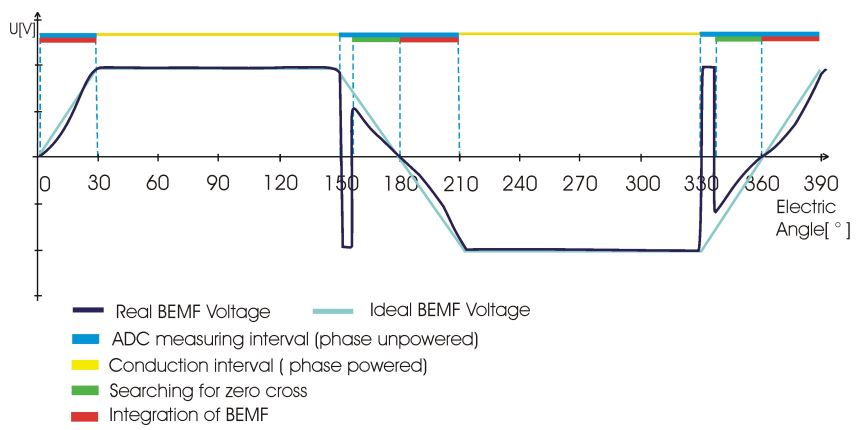
\includegraphics[width=\textwidth]{NXP_BackEMF_ElectricalRotation_OnePhase.JPG}
	\caption{Electrical rotation BEMF of one phase \cite{NXP_AN4597}}
	\label{fig:NXP_BackEMF_ElectricalRotation_OnePhase}
\end{figure}

The reason that this method works is because the flux measured at different speeds can be regarded as a constant for a certain motor \cite{NXP_AN4597}. \autoref{fig:NXP_BackEMF_Integration} shows the integrated voltage (flux) at different motor speeds.

\begin{figure}[H]
	\centering
	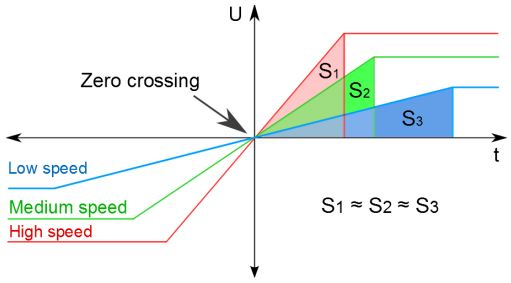
\includegraphics[width=0.6\textwidth]{NXP_BackEMF_Integration.JPG}
	\caption{Constant flux value with different motor speeds \cite{NXP_AN4597}}
	\label{fig:NXP_BackEMF_Integration}
\end{figure}

\subsection{BEMF and PWM}
The line shown in \autoref{fig:NXP_BackEMF_ElectricalRotation_OnePhase} only applies when one of the MOSFETs in the half-bridge is open constantly. However, sometimes you might want to drive the MOSFETs using a PWM signal. The resulting BEMF is shown in \autoref{fig:Microchip_PWM_BackEMF}. The choice can be made to either apply PWM to only the high-side MOSFETs (the MOSFETs connected to the positive terminal of the DC source) or to both the high- and low-side MOSFETs in a complementary fashion. The PWM frequency used in BLHeli\_32 is 24KHz by default while some even use 48KHz \cite{BLHeli_32_PWM_Frequency}. 

 \begin{figure}[H]
 	\centering
 	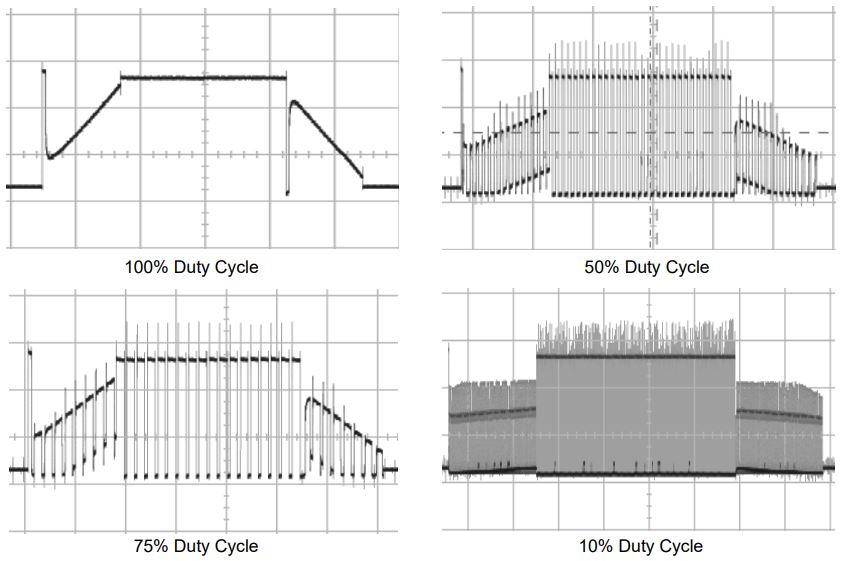
\includegraphics[width=\textwidth]{Microchip_PWM_BackEMF.JPG}
 	\caption{BEMF when driven the MOSFETs with PWM \cite{Microchip_AN857}}
 	\label{fig:Microchip_PWM_BackEMF}
 \end{figure}

ST describes a couple of PWM BEMF sampling methods in AN1946 \cite{ST_PWM_BEMF_sampling}. Some of these methods don't allow for the 100\% PWM duty cycle due to the nature of their sampling method. Which method is preferred for RC BLDC motors should be an experiment during the execution of the project.

Another method would be to place a buck converter in front of the MOSFET gates. This would show less of the PWM signal in the BEMF but would of course reduce the input voltage. During the execution of the project this method should be considered as an experiment. However, the direct PWM method is seen most often in controllers.

\subsection{Challenges with BEMF sensing}
The main challenges will be:
\begin{enumerate}
	\item Determine which BEMF sampling method for a PWM driven BLDC motor should be used \cite{ST_PWM_BEMF_sampling}.
	\item Determine the sampling frequency.
	\item Determine how the correct flux threshold for a certain motor should be determined.
	\item Determine the MOSFET PWM frequency to use.
	\item Determine how fast the motor can be accelerated/decelerated before the rotor gets out of sync with the commutation.
\end{enumerate}

\section{Starting a BLDC motor}
\subsection{Startup stages}
When a BLDC motor is stationary (or rotates very slowly) there is no or a negligible BEMF signal. Starting a BLDC motor consists of three stages \cite{ST_Starting_Sequence_BLDC}:
\begin{enumerate}
	\item Pre-positioning of the rotor.
	\item Starting ramp and accelerating the rotor. This stage decides the rotation direction of the rotor.
	\item Switching to control based on BEMF sensing.
\end{enumerate}

As stated in \cite{ST_Starting_Sequence_BLDC} most of the parameters involved with the startup stages are 'hard coded' and depend on the motor's physical parameters. One the BEMF signals is strong enough the BEMF based control can be started.

\subsection{Challenges with starting a BLDC motor}
The main challenges will be:
\begin{enumerate}
	\item Determine an efficient method for parameterizing the startup sequence.
	\item Determine when is a good moment to switch to the BEMF based control.
\end{enumerate}

\section{Simulation in Simulink}
\subsection{Simscape electrical}
Simulating the controller before implementing it in real life is a good method for getting a feel of some of the needed parameters.

Luckily the Simscape Electrical package for Simulink contains a BLDC motor block \cite{SimscapeElectrical_BLDC} (see \autoref{fig:SimscapeElectricalBldcBlock}). MathWorks also created a short video series demonstration how to use the BLDC motor block \cite{SimscapeElectrical_BLDC_VideoSeries}. 

\begin{figure}[H]
	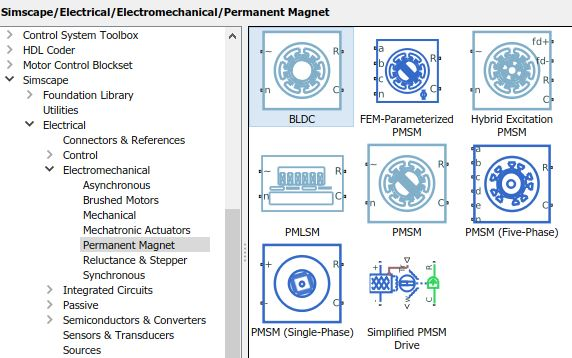
\includegraphics[width=0.6\textwidth]{SimscapeElectricalBldcBlock.JPG}
	\caption{BLDC motor block in the Simscape Electrical package for Simulink}
	\label{fig:SimscapeElectricalBldcBlock}
\end{figure}

\subsection{Challenges with simulation in Simulink}
The main challenges will be:
\begin{enumerate}
	\item Determining what good parameters are to simulate a typical BLDC motor used in a drone.
	\item Making the model flexible enough to allow for easy experimentation.
	\item Keeping in mind that the model should be relatively easy to transfer to the real world.
	\item Will a transfer-function based system or a state-space based system be created.
	\item Determine which properties of the motor can be directly measured and which can be inferred.
\end{enumerate}

\section{Implementation in real life}
After the Simulink model is created and tested it is time to transfer it to the real world.

\subsection{Circuit design}
The prototype ESC will have a serial input, just like the currently used ESCs for FPV drones. It will, however, not necessarily use the DShot protocol since this is just a prototype.

The first thing to do is to design the circuit. The circuit will consist of:
\begin{itemize}
	\item Six MOSFETs for the six-step commutation
	\item A microcontroller
	\item A circuit for getting the BEMF signals back to the microcontroller.
	\item Protection circuitry.
	\item Miscellanious components
\end{itemize}

\subsection{Translating the Simulink model into code}
Before the circuit can be tested, code should be written for the microcontroller. Simulink can generate code for microcontrollers. If the generated code is not (easily) usable for the microcontroller, the choice can be made to implement the code from scratch.

It will be important to implement the control loop with the correct sampling frequency, keeping in mind the workload and frequency of the microcontroller.

\subsection{Challenges with the implementation in real life}
The main challenges will be:
\begin{enumerate}
	\item Choosing the correct components for the physical prototype.
	\item Designing the circuit.
	\item Investigate whether or not the generated code from Simulink can be used.
	\item Correctly implement the discrete controller.
	\item If a MOSFET driver IC is used, the possible delay between input and output should be taken into consideration.
\end{enumerate}

\chapter{Deliverable}


\printbibliography


\end{document}